\subsection{Introduction}
Spike trains can be analyzed by exploiting several kinds of techniques, according
to the aim of the analysis. In particular, it might be interesting to study the
behaviour of a recording site after an external stimulation. Notice that this kind
of analysis becomes more and more relevant as it is extended to multiple channels, for
instance in order to study how different neurons react to the same stimulus. Other
interesting analyses might consist in comparing the responses from several channels or from corresponding channels in different subjects, establishing proper metrics to assess similarity
and correlation.

\subsection{Post Stimulus Time Histogram}
The Post Stimulus Time Histogram (PSTH) is a vital tool to characterize neural spike trains
in response to a stimulus. In general, the response of a certain neuron
for a repeated given stimulus is not identical, but it tends to change, due to adaptation.
\begin{figure}[H]
    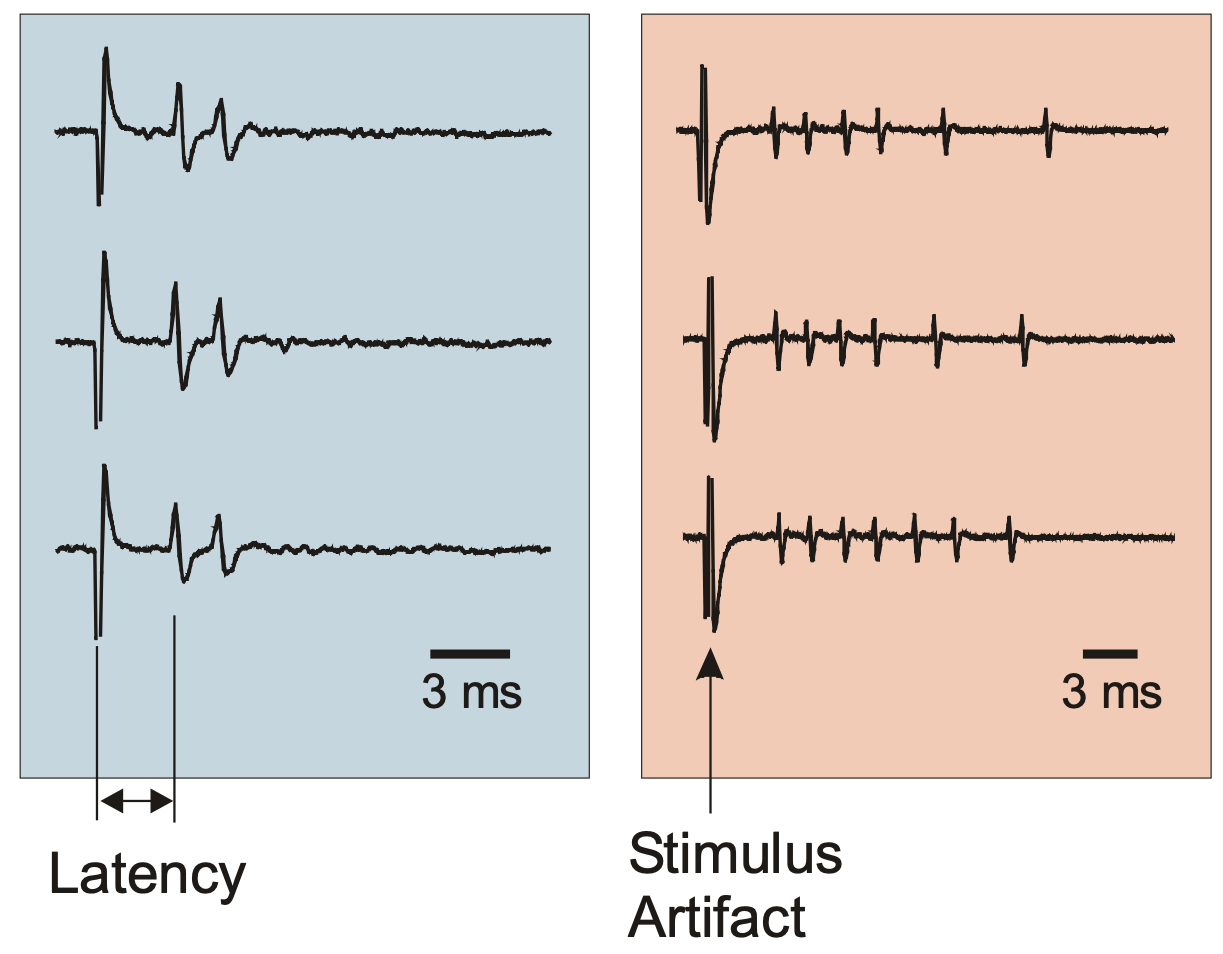
\includegraphics[scale=0.22]{8_1}
    \centering
\end{figure}
In these images the big spike is due to the electrical stimulation. What comes after is the response. What has to be found is the latency between the stimulation time point and the moment of response. The higher is the stimulus, the better is also the response.\\
To build a PSTH, a certain time window is isolated after the occurrence of the stimulus and it is divided into several equally long bins. Then, the total number of spikes in each bin is counted and reported into the histogram, as shown in the figure below.
\begin{figure}[H]
    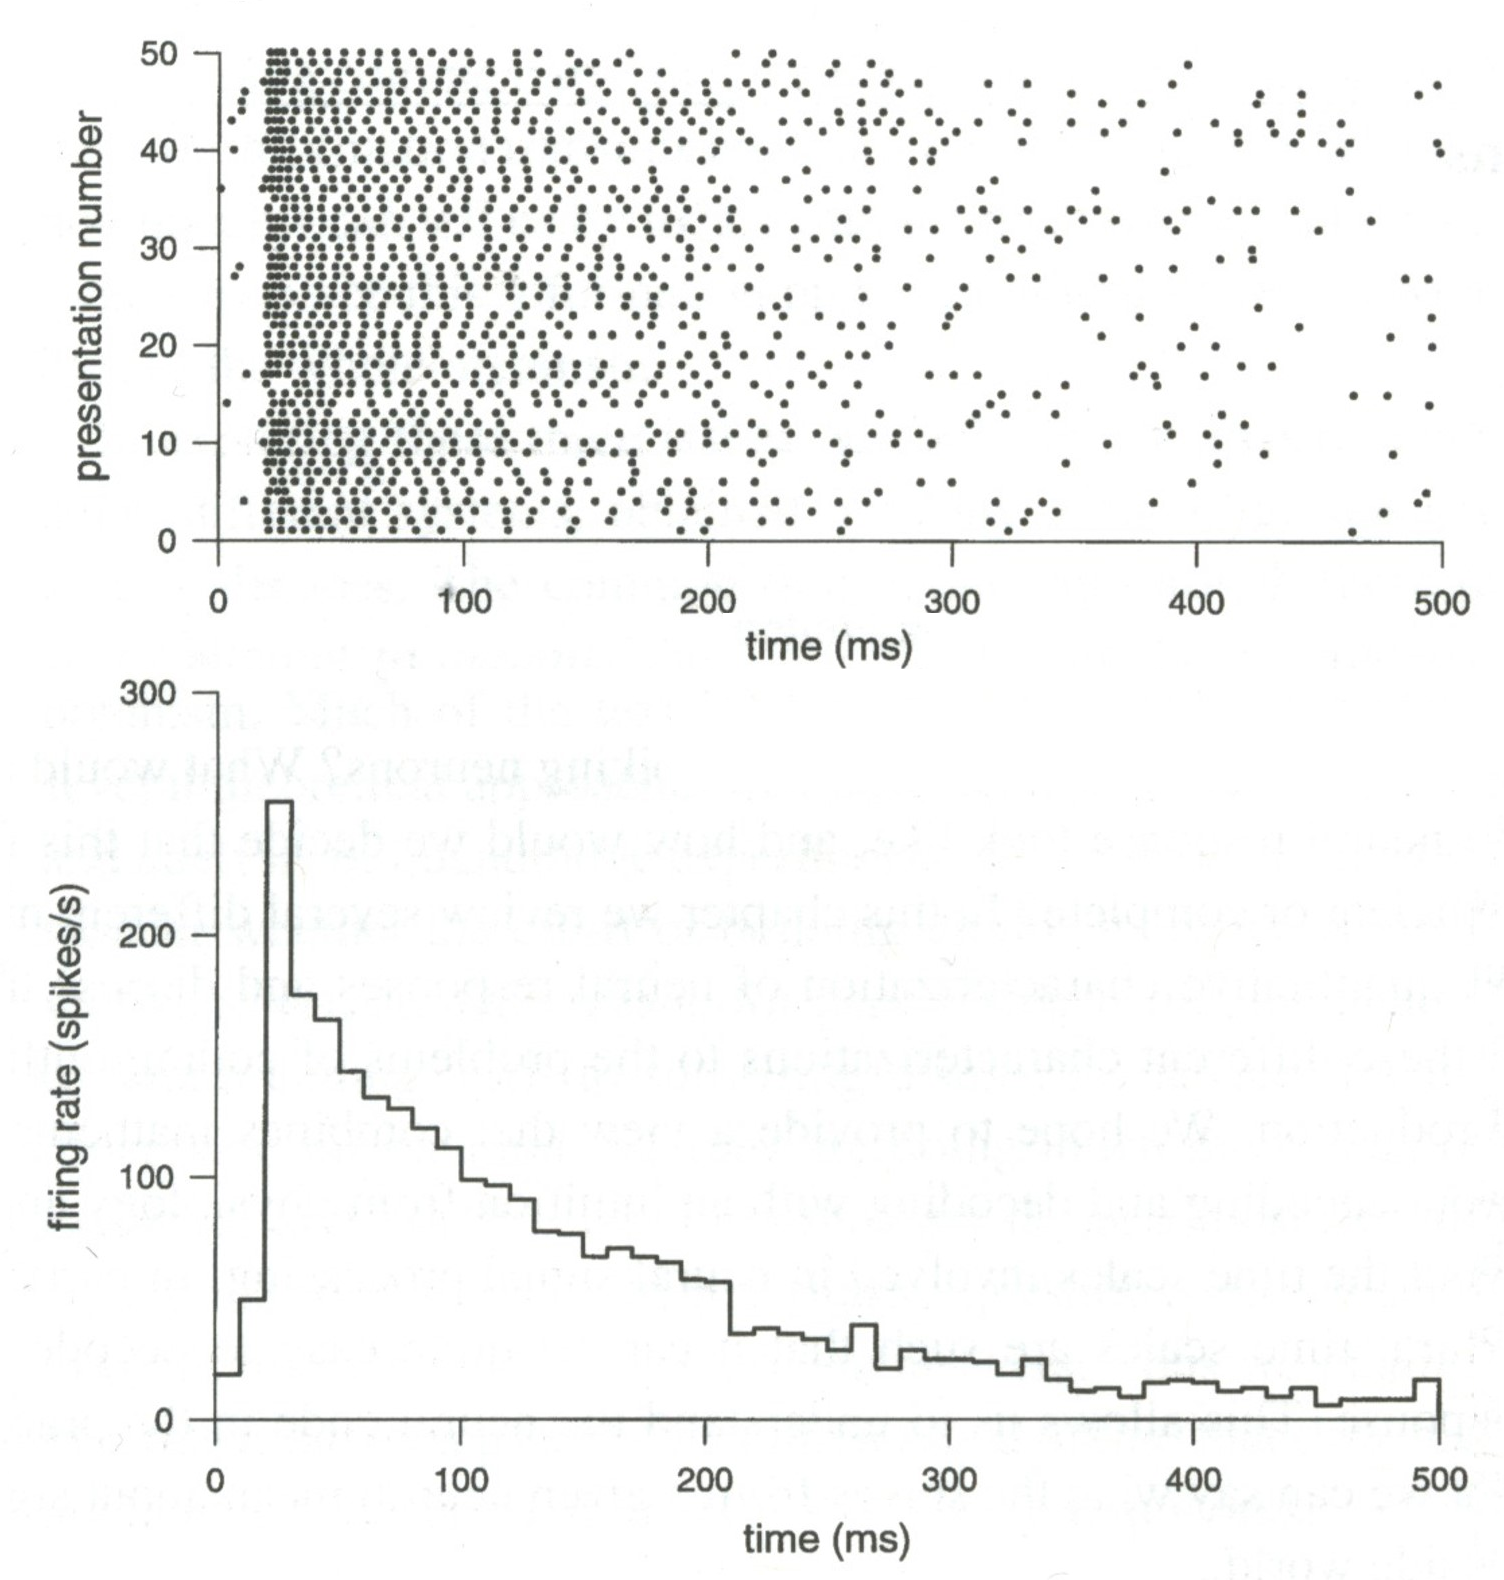
\includegraphics[scale=0.28]{8_2}
    \centering
\end{figure}
On the x axis there are the bins in which the whole time interval in which the measurement has been done has been divided. On the y axis there is average number of spikes in each bin, following stimulus presentation and normalization to the number of presentations and the bin size. Normalized in this way, the PSTH gives the \textbf{firing rate} or the \textbf{probability of firing per unit of time}.\\
Generally, after after being stimulated, a neuron can exhibit two different responses:
\begin{itemize}
    \item \textbf{Early response:} it occurs in the first \(50\,ms\) after the stimulus
          and includes the direct activation of the neuron.
    \item \textbf{Late (or delayed) response:} it occurs at least after \(50\,ms\) and up to
          \(400\,ms\), representing a reverberating response.
    \begin{figure}[H]
    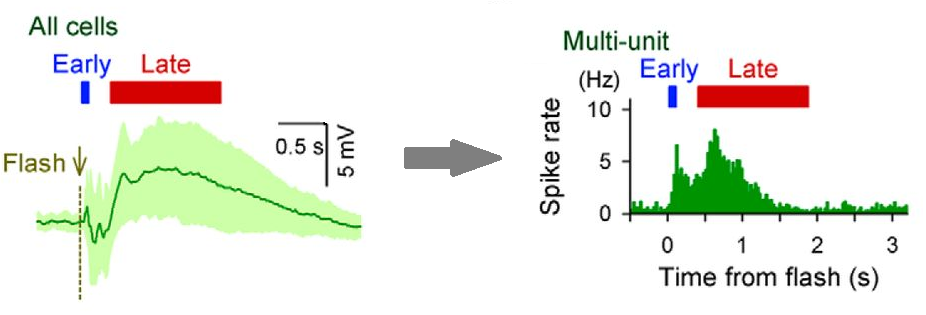
\includegraphics[scale=1.1]{8_3}
    \centering
\end{figure}
\end{itemize}
It can be said that the early response is definitely more reliable than the late
response, as the second one might be influenced by noise.\\
A way to better focus on the early response direct activation consists in chemically blocking the synapses.
\begin{figure}[H]
    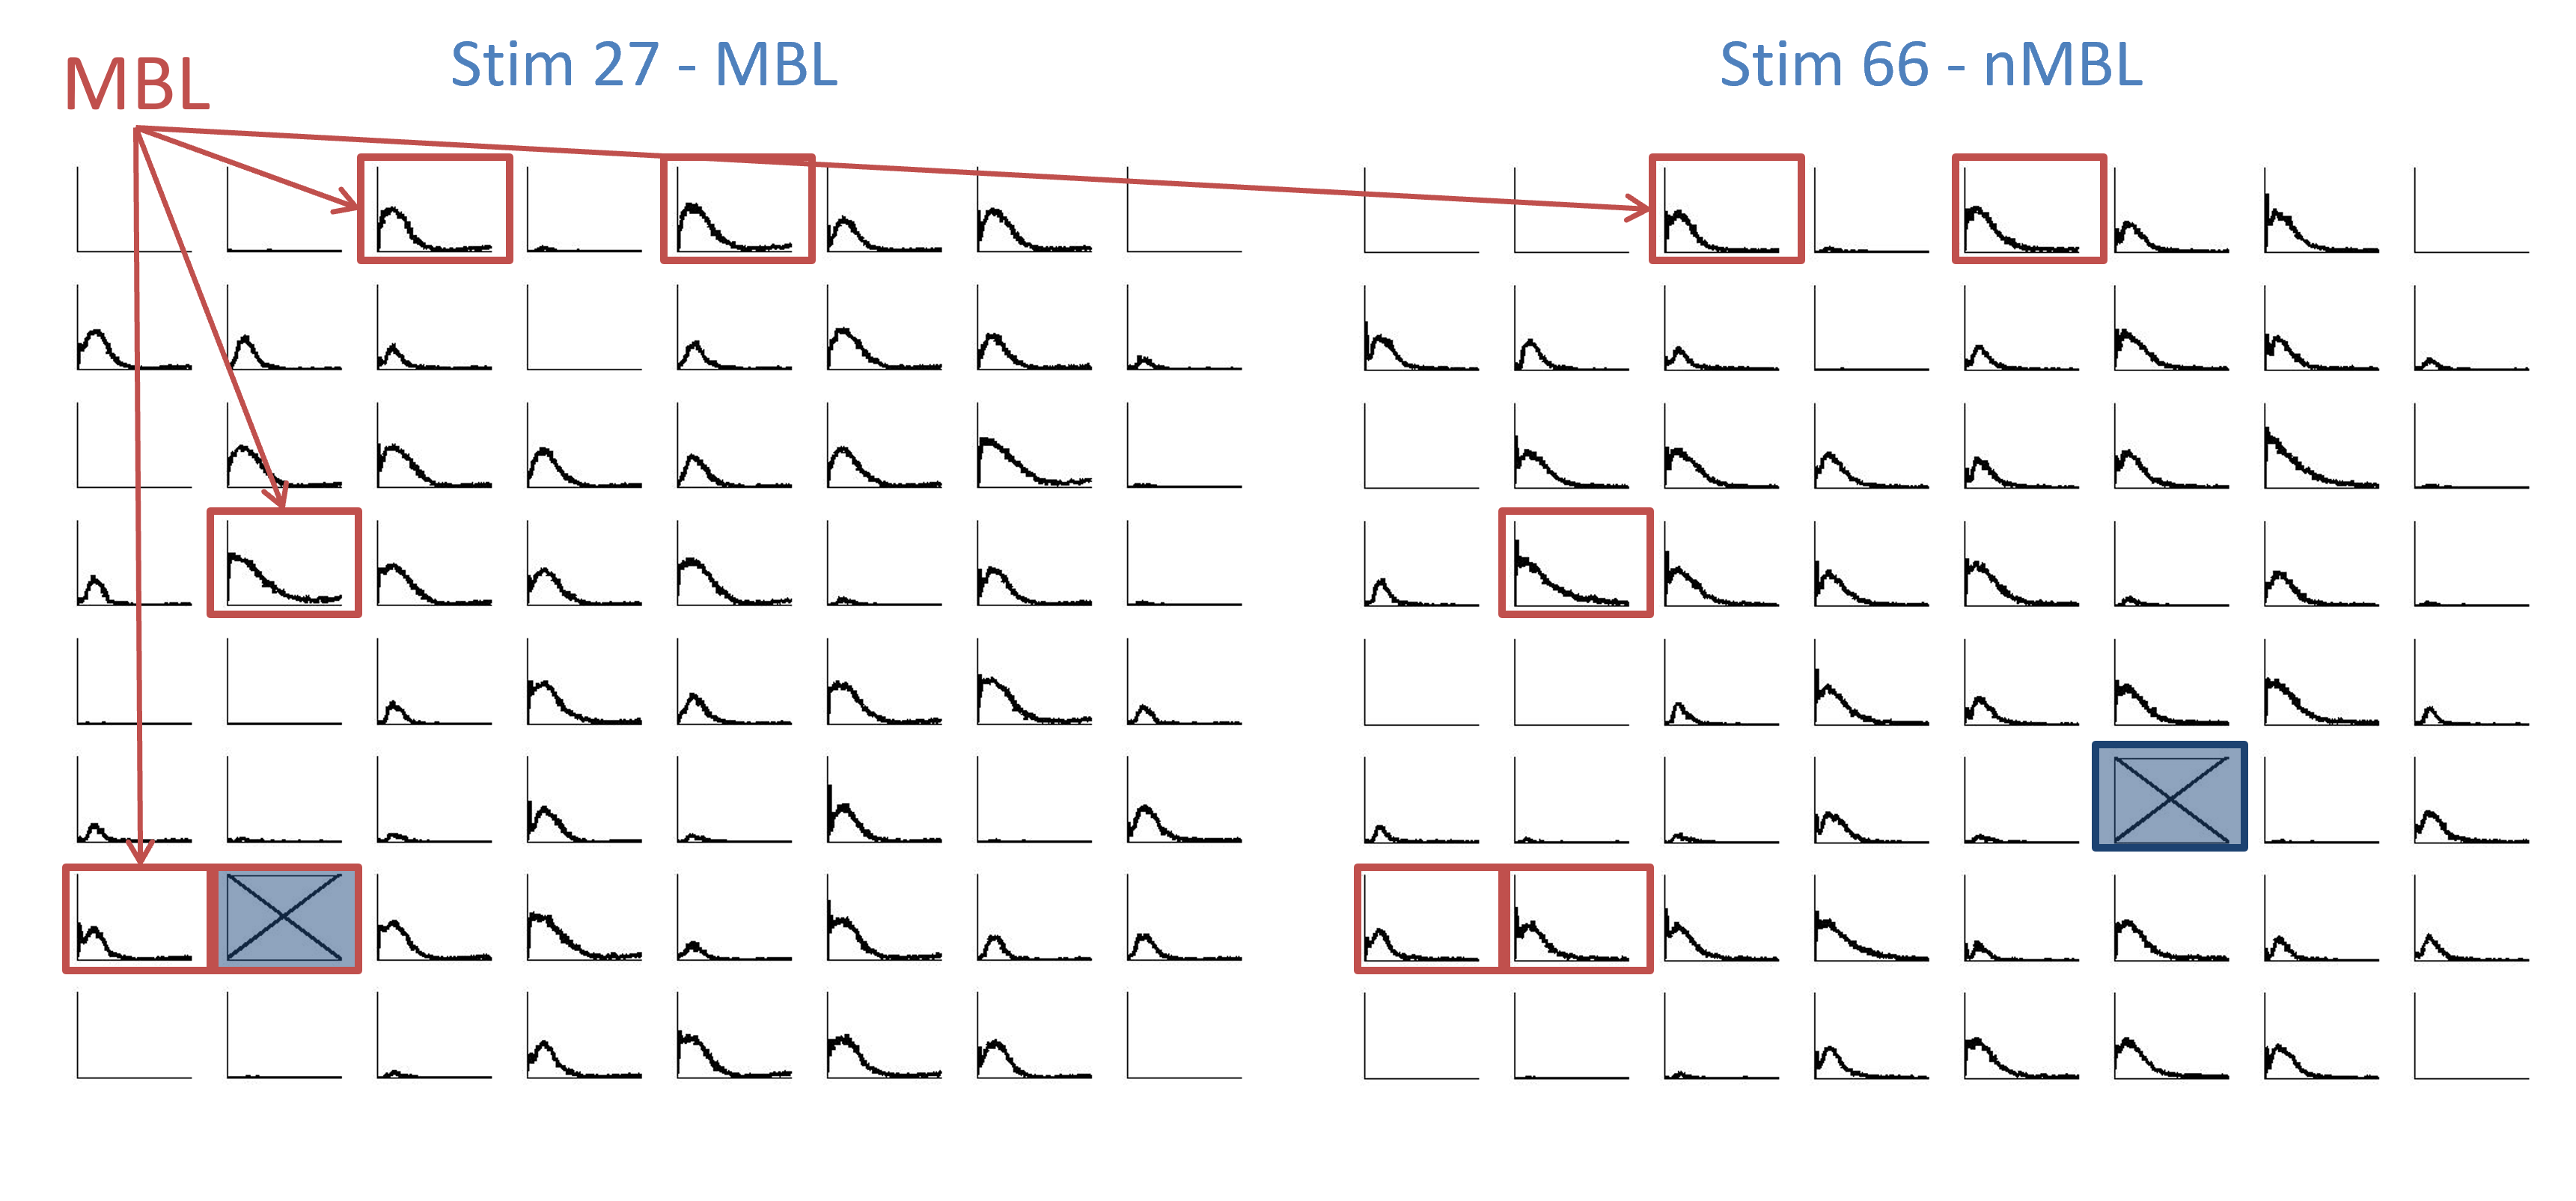
\includegraphics[scale=0.25]{8_4}
    \centering
\end{figure}
These figures represent the pharmacological response of cells in which the synapses are working (A and C) and are blocked (B and D). We can see that the direct activation is present in both images because it is related to monosynaptic responses (the stimulation and the response are related to the same neuron). On the other hand, the other peaks are present only in the C plot: they are due to the response events triggered by the stimulation in nearby neurons, that in the first case can communicate and send the information to the electrode, but in the other have been blocked, hence their response channel isn't working.\\
NB: color codes: yellow = positive amplitudes and blue = negative amplitudes.\\
Moreover, also PSTH raster plots can be realized, in which the response recorded by many channels is plotted. In this case a PSTH for each channel is built and, if the activity is similar in the different channels, the network PSTH can be derived.\\
PSTH raster plots might also represent a valuable tool to individuate Major Burst
Leaders (MBLs), as a PSTH highlights the rapidity of a neuron to produce a response. In the
following picture a histogram for each channel of an array of electrodes is represented,
according to the physical layout of the electrodes, and the MBLs are highlighted in red.
\begin{figure}[H]
    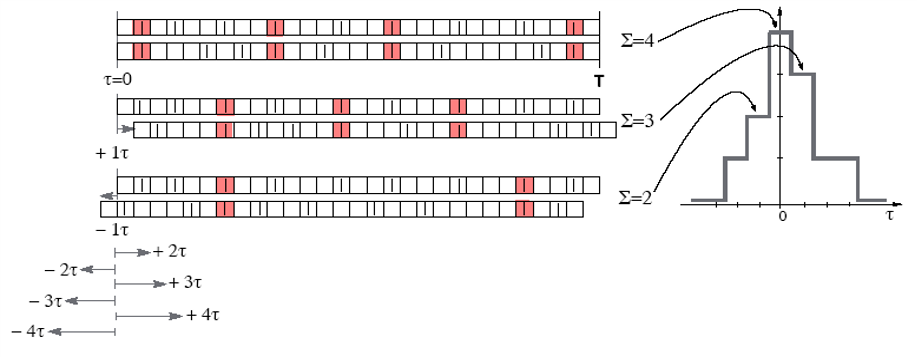
\includegraphics[scale=0.6]{8_5}
    \centering
\end{figure}
\subsection{Cross-Correlation}
The cross-correlation between spike trains is a fundamental metric, as it is capable
to highlight synchronization phenomena at the network level. This metric
can alternatively be computed starting from the spike trains or the burst event trains (in which a burst is found using only its first spike).\\
Different steps are necessary to find a \textbf{cross-correlogram} (i.e., a cross-correlation histogram):
\begin{enumerate}
    \item Identify a \textbf{reference train} and a \textbf{target train}, denoted respectively as \(x\) and \(y\).
    \item Divide the two trains into equally spaced bins small enough to contain at most one spike. In this way a histogram that tells us how the spikes in the reference are related to the spikes in the target can be built. To do it, spikes of the target train are projected on the reference spike train.  A time delay \(\tau\) is applied as a variable shift between the two trains. The position of the projected spike becomes the zero of a new time axis, which has to be divided in bins again in order to count the spikes inside them.
    \item At the end, an histogram is obtained, which has values between \(-T\) and \(T\) on the \(x\) axis and \(C_{xy}(\tau)\) on the \(y\) axis, that is the cross correlation between the spike trains. 
\end{enumerate}
Notice that by switching the reverse and the target trains, the same plot is obtained,
but reversed in the horizontal time axis.\\
When \(\tau = 0\), the reference spike train is synchronized with the target spike train: it means that the cross-correlation is high, hence a big central peak and very low lateral ones are expected (\textbf{auto-correlation}).
\begin{figure}[H]
    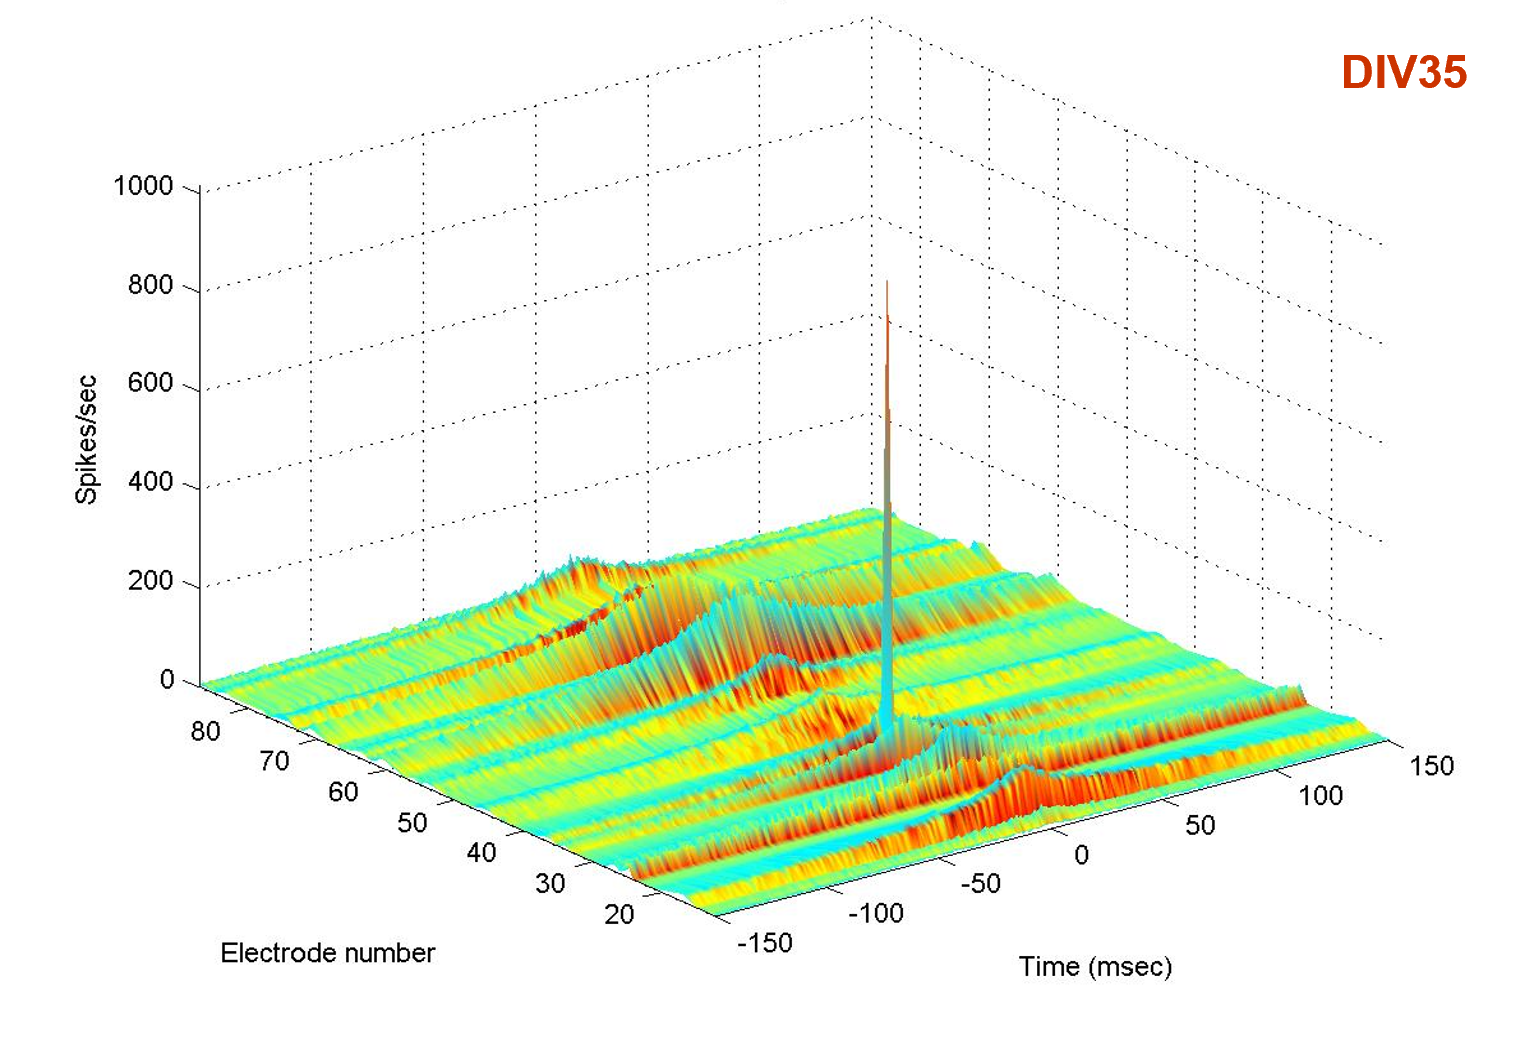
\includegraphics[scale=0.9]{8_6}
    \centering
\end{figure}
From a mathematical point of view, the cross-correlation \(C_{xy}\) can be formalized
as follows:
\begin{align*}
    C_{xy}(\tau)
    =\sum_{s=1}^{N_x}\sum_{t_{i}=(\tau-\Delta{\tau}/2)}^{(\tau+\Delta{\tau}/2)}x(t_s)y(t_s-t_i)
\end{align*}
A normalization term can be easily added in order to obtain
a cross-correlation value in the \([0, 1]\) range:
\begin{align*}
    C_{xy}(\tau)
    =\frac{1}{\sqrt{N_xN_y}}\sum_{s=1}^{N_x}\sum_{t_{i}=(\tau-\Delta{\tau}/2)}^{(\tau+\Delta{\tau}/2)}x(t_s)y(t_s-t_i)
\end{align*}
where \(N_x\) is the total number of spikes in the reference train and \(N_y\) is the
total number of spikes in the target train. The previously described properties of
\(C_{xy}(\tau)\) can be summarized as:
\begin{itemize}
    \item \(0\le{C_{xy}(\tau)}\le{1}\rightarrow\) thanks to the normalization
    \item \(C_{xy}(\tau)=C_{yx}(-\tau)\rightarrow\) symmetry between target and reference trains
\end{itemize}
Also other kinds of normalization factors can be used, even if they can introduce some problems:
\begin{equation*}
    N_f = \frac{1}{N_x} \hspace{0.5cm} N_f=\frac{1}{N_y} \hspace{0.5cm} N_f=\frac{1}{N_xN_y}
\end{equation*}
Auto-correlation is often used to test the correct functioning of a cross-correlation
algorithm:
\begin{align*}
    C_{xx}(\tau)
     & =\frac{1}{\sqrt{N_xN_x}}\sum_{s=1}^{N_x}\sum_{t_{i}=(\tau-\Delta{\tau}/2)}^{(\tau+\Delta{\tau}/2)}x(t_s)x(t_s-t_i) \\
     & =\frac{1}{N_x}\sum_{s=1}^{N_x}\sum_{t_{i}=(\tau-\Delta{\tau}/2)}^{(\tau+\Delta{\tau}/2)}x(t_s)x(t_s-t_i)
\end{align*}
\begin{figure}[H]
    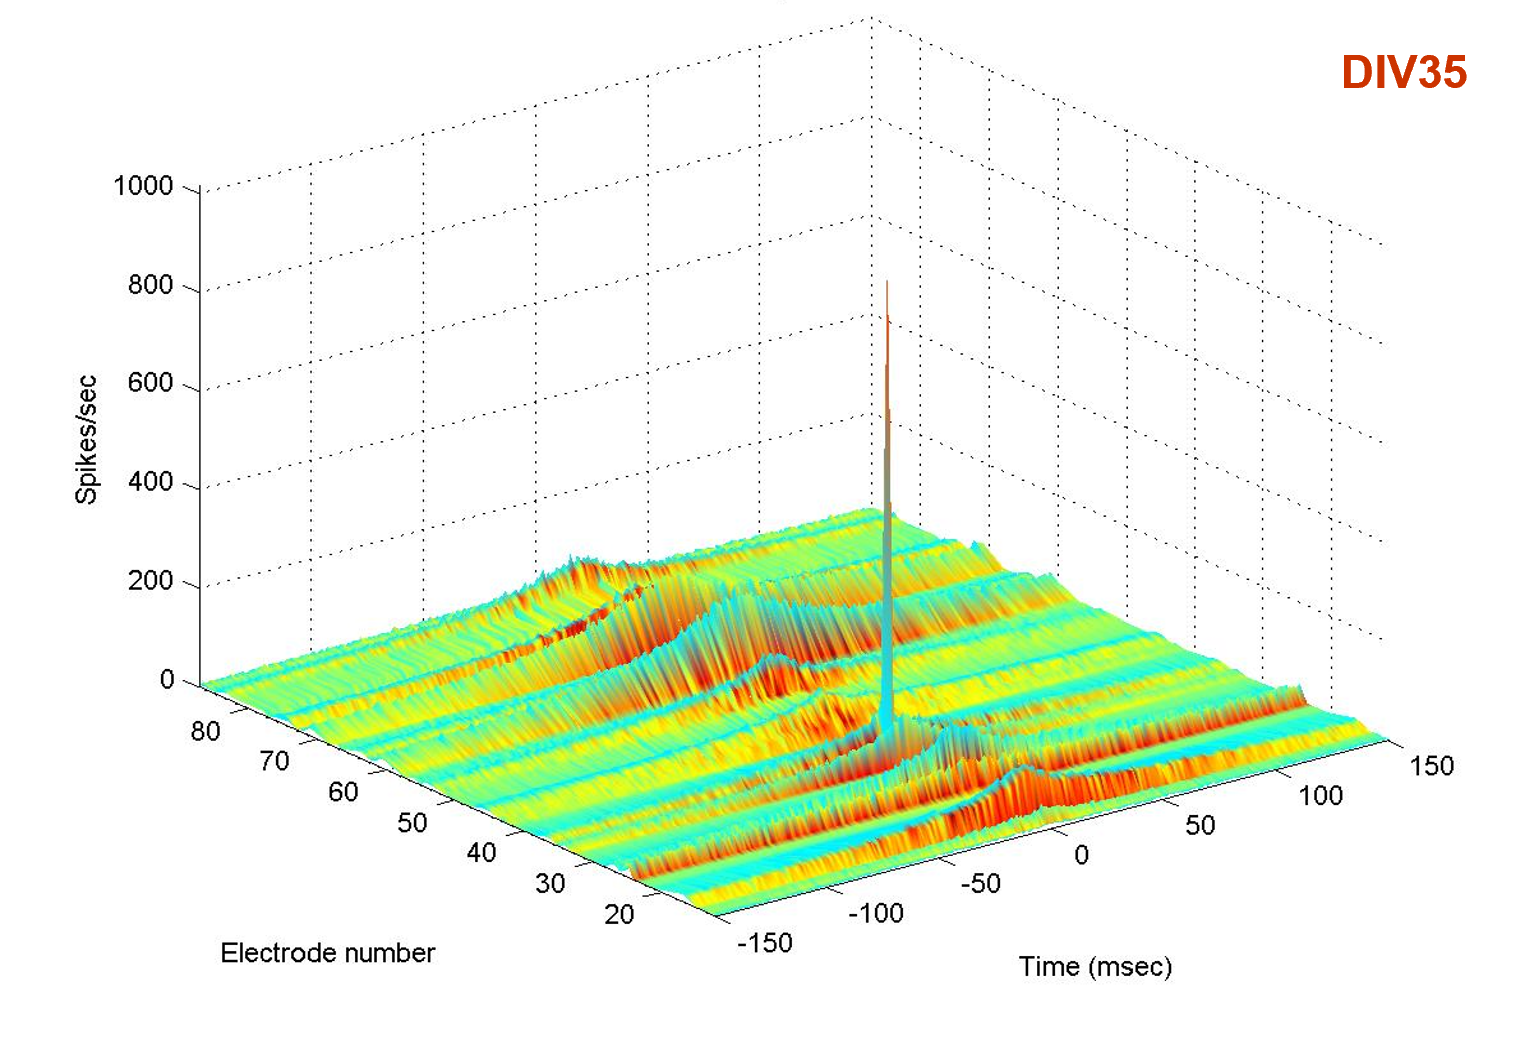
\includegraphics[scale=0.9]{8_7}
    \centering
\end{figure}
\subsubsection{Meaningful Parameters}
From the cross-correlation, some parameters can be extracted.
\begin{itemize}
    \item \textbf{Mean-correlogram}: The mean-correlogram can be computed to assess how one channel is correlated to all of the others:
    \begin{align*}
        C_x(\tau)=\frac{1}{n-1}\sum_{y=1}^{n}C_{xy}(\tau)
    \end{align*}
    To find it, the auto-correlation is not considered.
    \item \textbf{Correlation Function in 0}: It is the area under the curve limited by the temporal dimension of the bin centered in 0 (\(\Delta\tau\)). Since sometimes this quantity is very small, also a higher number \(k\) of bins around 0 can be considered.
    \begin{align*}
        C(0)=\sum_{\tau=-k(\Delta\tau/2)}^{k(\Delta\tau/2)}C_{xy}(\tau)
    \end{align*}
    \item \(\mathbf{C_{peak}}\): It represents the value of the cross-correlogram in
    an area around the maximum detected peak. This is computed in order to quantify the
    correlation level among all the recording channels. 
    \begin{align*}
        C_{peak}=\sum_{\tau=\tau_{peak}-k(\Delta\tau/2)}^{\tau_{peak}+k(\Delta\tau/2)}C_{xy}(\tau)
    \end{align*}
    \item \textbf{Peak Latency}: It is the distance of the maximum peak from the zero, and it can be interpreted as the delay of an estimated functional connection or alternatively as the directionality of the connection between two sources. \\
    Two channels can be considered as synchronized whenever the central peak is centered in zero, implying a very small peak latency.
    \begin{figure}[H]
        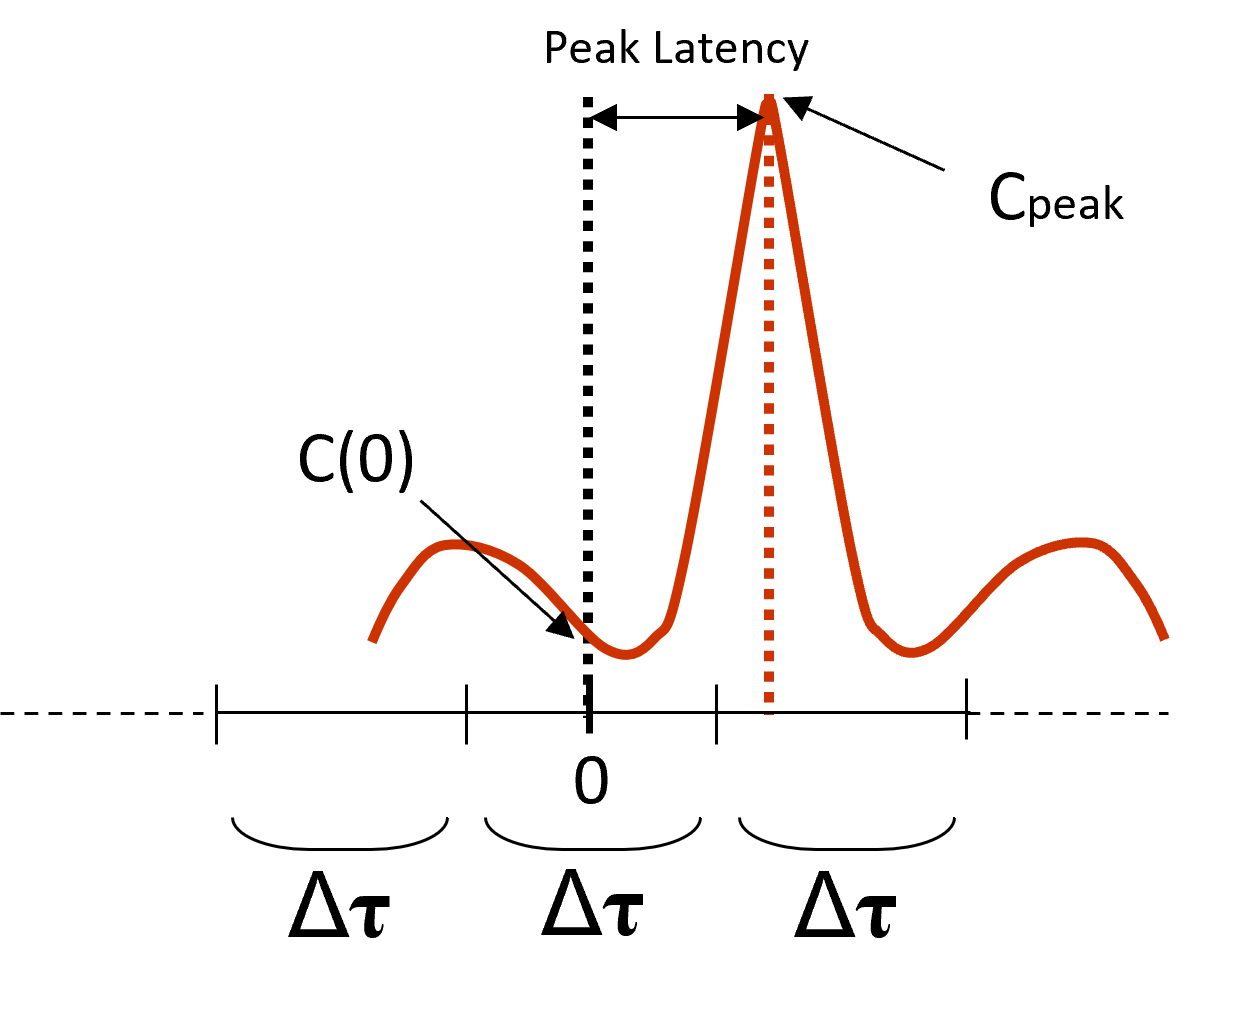
\includegraphics[scale=0.7]{8_8}
        \centering
    \end{figure}
    \item \textbf{Coincidence Index}: The Coincidence Index, often indicated with \(CI\), is a percentage indicator of the synchronization level between two channels. It can be defined both for 0 and for the correlation peak.
    \begin{align*}
        CI_{zero} & = \frac{C(0)}{\sum_{\tau=-T}^{T}C_{xy}(\tau)}     \\
        CI_{peak} & = \frac{C_{peak}}{\sum_{\tau=-T}^{T}C_{xy}(\tau)}
    \end{align*}
    Notice that the denominator \(\sum_{\tau=-T}^{T}C_{xy}(\tau)\) represents the total
    area under the cross-correlogram curve.
\end{itemize}
\subsection{The Pearson's Correlation Coefficient}
The Pearson's Correlation Coefficient is another tool used to indicate the correlation between two variables \(X\) and \(Y\) - i.e. the degree to which the variables are related to each other.
When computed in a sample, the Pearson's Correlation Coefficient is indicated as \(r\).
Notice that it reflects the degree of linear relationship between two variables,
in the \([-1;+1]\) range:
\begin{itemize}
    \item \(\mathbf{r=+1}\): there is a \textbf{perfect positive linear
              relationship} between the variables \(X\) and \(Y\Rightarrow\) high scores on
          the X-axis are associated with high scores on the Y-axis.
    \item \(\mathbf{r=-1}\): there is a \textbf{perfect negative linear
              relationship} between the variables \(X\) and \(Y\Rightarrow\) high scores on
          the X-axis are associated with low scores on the Y-axis.
    \item \(\mathbf{r=0}\): there is \textbf{no linear
              relationship} between the variables \(X\) and \(Y\).
\end{itemize}
Generally, the Pearson's Correlation Coefficient is computed as follows:
\begin{align*}
    r=\frac{\sum_{i=1}^{N}(x_i-\overline{x})(y_i-\overline{y})}{\sqrt{\sum_{i=1}^{N}(x_i-\overline{x})^2\sum_{i=1}^{N}(y_i-\overline{y})^2}}
\end{align*}
In the neuroscience field, the Pearson's Correlation Coefficient has been proposed
as a measure of synchronization among different units of a neuronal network.
In this case, \(r\) can be computed in a much easier way:
\begin{align*}
    r=\frac{N\sum_{i=1}^{N}x_{i}y_{i}-N_{x}N_{y}}{\sqrt{N_{x}(N-N_{x})}\sqrt{N_{y}(N-N_{y})}}
\end{align*}
where \(N_x=\sum{x_i}\) is the number of spikes in the \(x\) train and \(N_y=\sum{y_i}\) is the number of spikes in the \(y\) train.
\subsection{Visualization Tools}
Various graphic tools can be employed to visualize the correlation degree of several
recording channels in a neuronal network.
\subsubsection{Multi-Channel Raster Plot} 
This kind of plots allows the visual inspection
of several channels at the same time, making easy to see if the spike trains coming
from different recording sites are similar one to another. Although this tool is
pretty simple to implement, it becomes ineffective in the case of correlations that are
not immediately visible.
\begin{figure}[H]
    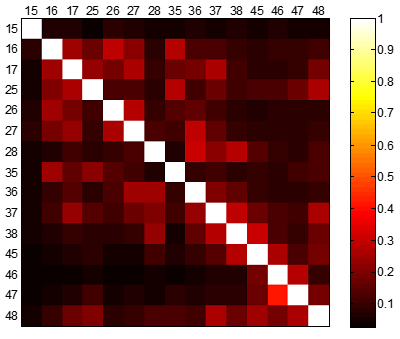
\includegraphics[scale=0.7]{8_9}
    \centering
\end{figure}
\subsubsection{Correlation Matrix Plot} 
The correlation matrix is usually computed for
the zero point, indicated as \(C(0)\), and for every possible pair of
recording channels. The obtained values are then plotted by using a heatmap. Notice that the
main diagonal exhibits a maximum correlation, as it represents the auto-correlation
for each channel. Moreover, the resulting matrix is symmetrical, due to the properties of the cross-correlation coefficient.
\begin{figure}[H]
    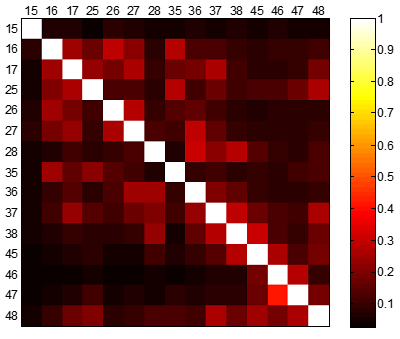
\includegraphics[scale=0.7]{8_10}
    \centering
\end{figure}
\subsubsection{Connectivity Map} 
This method allows to plot a topological mapping of the
connections between the sources, according to their activity. Each node is drawn,
according to its position on the MEA. Then, the correlation \(C(0)\) between each pair
of the recording channels is computed and a connecting line is added if \(C(0)\)
overcomes an arbitrary threshold - i.e. \(C(0)>0.2\). In addition, the thickness of
the line is proportional to the degree of correlation between the two nodes.
Notice that it is common to observe stronger connections between nodes close to
each other.
\begin{figure}[H]
    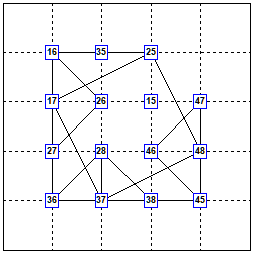
\includegraphics[scale=0.9]{8_11}
    \centering
\end{figure}

\subsection{Appendix}
\subsubsection{Self-Organized Criticality}
\textbf{Self-Organized Criticality (SOC)} is a theory in statistical physics, aimed at explaining the ubiquitous presence in nature of spatial fractals and fractal time series, also known as "\(1/f\) fluctuations" or "\(1/f\) noise".\\
Several phenomena in nature are scale-free, i.e., they are not characterized by a specific size or duration, but they display a power law distribution of spatial and/or temporal quantities(e.g. earthquakes, biological evolution, forest fires, etc). 
\begin{figure}[H]
    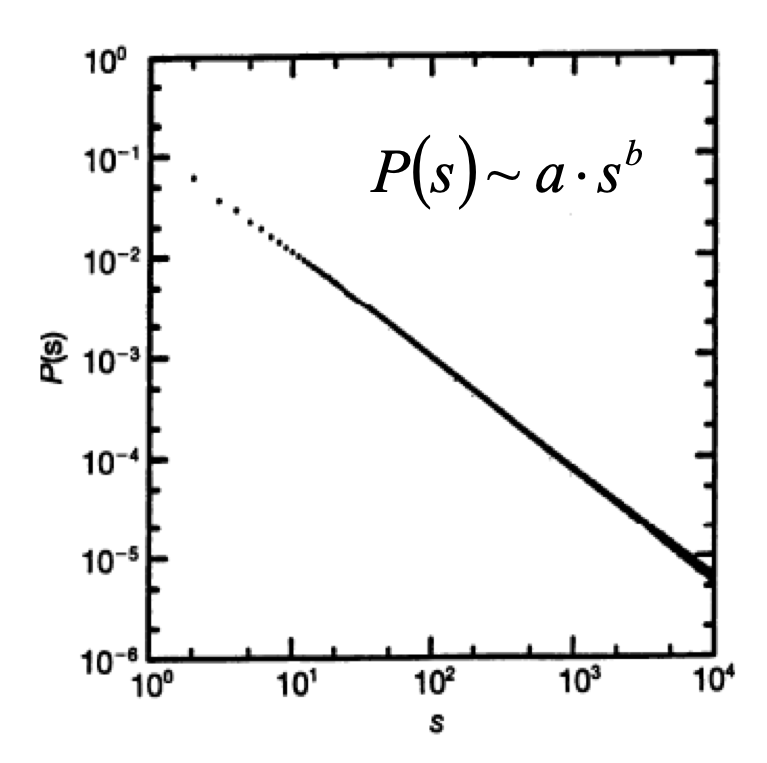
\includegraphics[scale=0.5]{8_12}
    \centering
\end{figure}
According to the SOC theory, dynamical systems composed of many nonlinear interacting units self-organize in a \textbf{critical state}, where even a small perturbation can lead to events of any dimension. Such critical state has many good properties, such as long range spatial and temporal correlations.\\
The prototypical example of self-organized critical system is the sandpile model, presented by Bak, Tang and
Wiesenfeld in 1987, and whom the term "neuronal avalanches" originates from. As it is a system composed of many interacting threshold elements (i.e., neurons) forming a network through a self-
organizing process, also the brain may be regarded as a self-organized critical system.\\
Three main states can be identified in these systems:
\begin{itemize}
    \item \textbf{Subcritical}
    \item \textbf{Critical}
    \item \textbf{Supercritical}
\end{itemize}
The difference between them is the slope of the power law, that is close to -1 for the critical state:
\begin{figure}[H]
    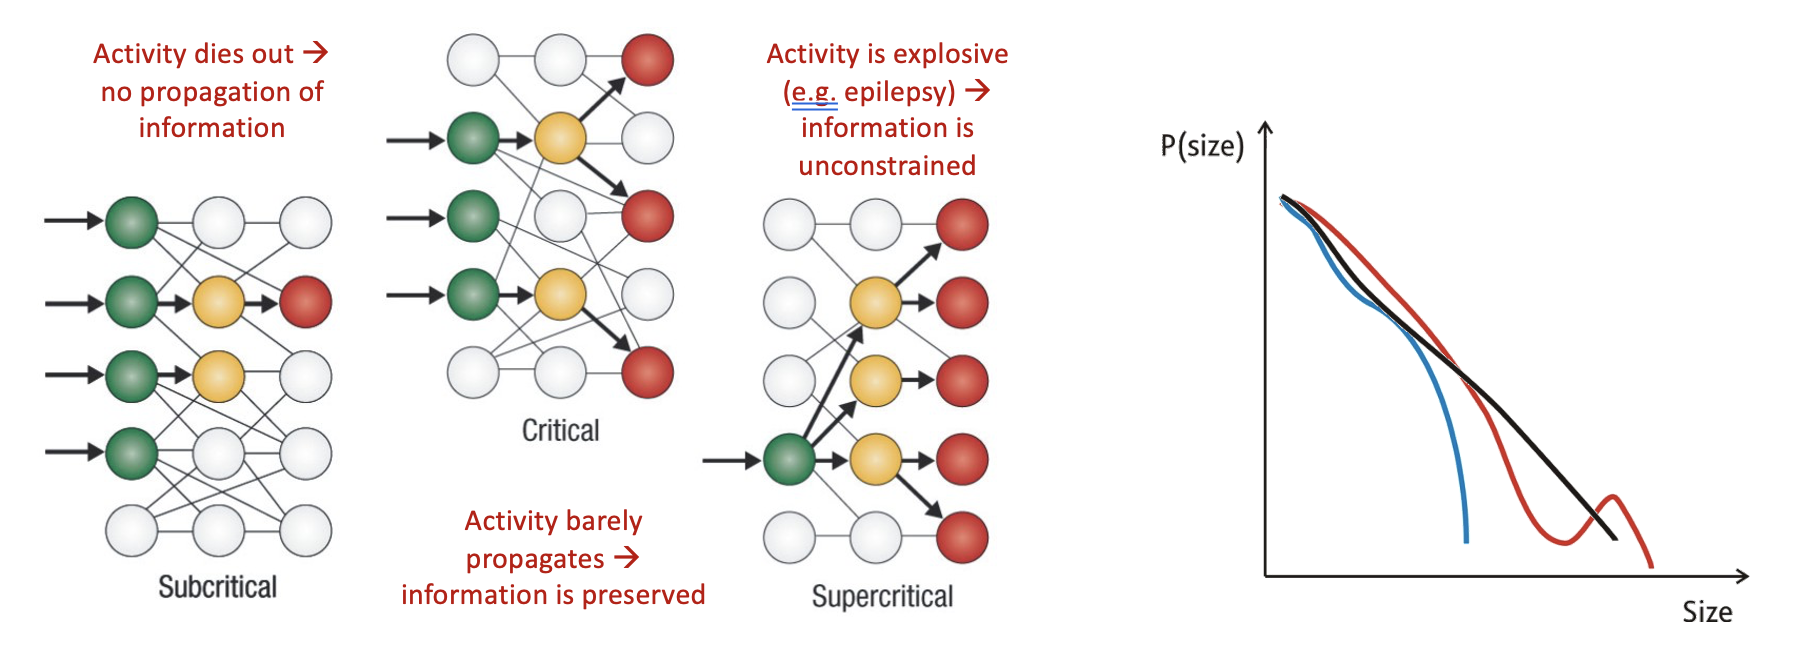
\includegraphics[scale=0.45]{8_13}
    \centering
\end{figure}
Beggs and Plenz were the first who demonstrated that in vitro brain slices display neuronal avalanches, whose size (and lifetime) distribution follows a power-law behavior. The presence of critical neuronal avalanche has been further confirmed in in vivo experiments:
\begin{figure}[H]
    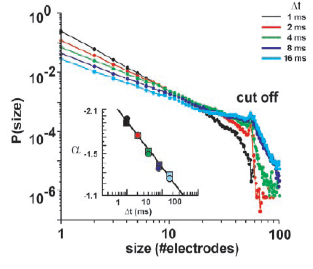
\includegraphics[scale=0.6]{8_14}
    \centering
\end{figure}
It can be observed that the slope of the probability is preserved: it is close to -1.5, that belongs to critical state.\\
A \textbf{neuronal avalanche} can be defined as an event of widespread spontaneous electrical activity, preceded and followed by a silent period. It involves all the electrodes. The burst is a specific case of avalanche.\\
Neuronal avalanches can be detected:
\begin{enumerate}
    \item Dividing the time axis into bins
    \item Performing different measurements related to the size of the avalanche (number of spikes, electrodes, bins involved).
\end{enumerate}
The time window used to bin the spiking activity has to be adjusted according to the signal's timescale (i.e. average inter-event interval): LFP\(\simeq4\,ms\), spikes\(\simeq0.2\,ms\).
\begin{figure}[H]
    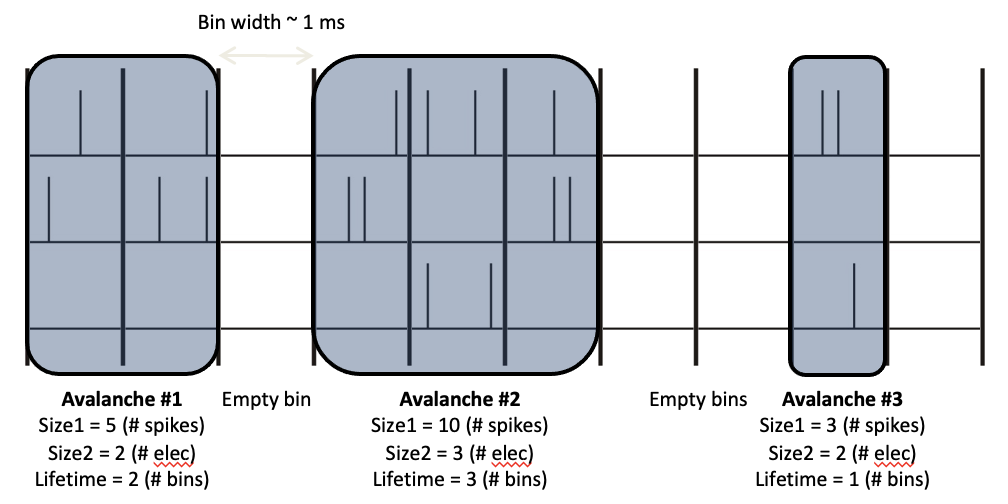
\includegraphics[scale=0.7]{8_15}
    \centering
\end{figure}
The number of avalanches per minute increases as the network develops. Once the culture has reached the mature stage (about 30 DIV), it shows a preferred behavior. Some networks in vitro organize themselves also in the subcritical or in the supercritical states.\\
The different states can also be correlated with bursting and spiking activity:
\begin{itemize}
    \item Criticality is correlated with average synchronization of bursts among electrodes and poor random spiking activity.
    \item Subcritical distribution shows low-level of synchronization and a few bursts.
    \item Supercritical distribution displays high-level of synchronization and many bursts.
\end{itemize} 
Therefore, the activity can also be manipulated using pharmacological methods, such as BIC or ACh: ACh enhances the persistent spiking activity of individual neurons by means of a strong depolarization of the resting membrane potential, causing desynchronization and disaggregation of activity, while BIC is a strong antagonist of the inhibitory synaptic receptors GABA that causes a strong enhancement of burstiness and synchronization.
In the first case, the distribution switches from a critical to a subcritical behavior, whereas under BIC the distribution is markedly supercritical.
\begin{figure}[H]
    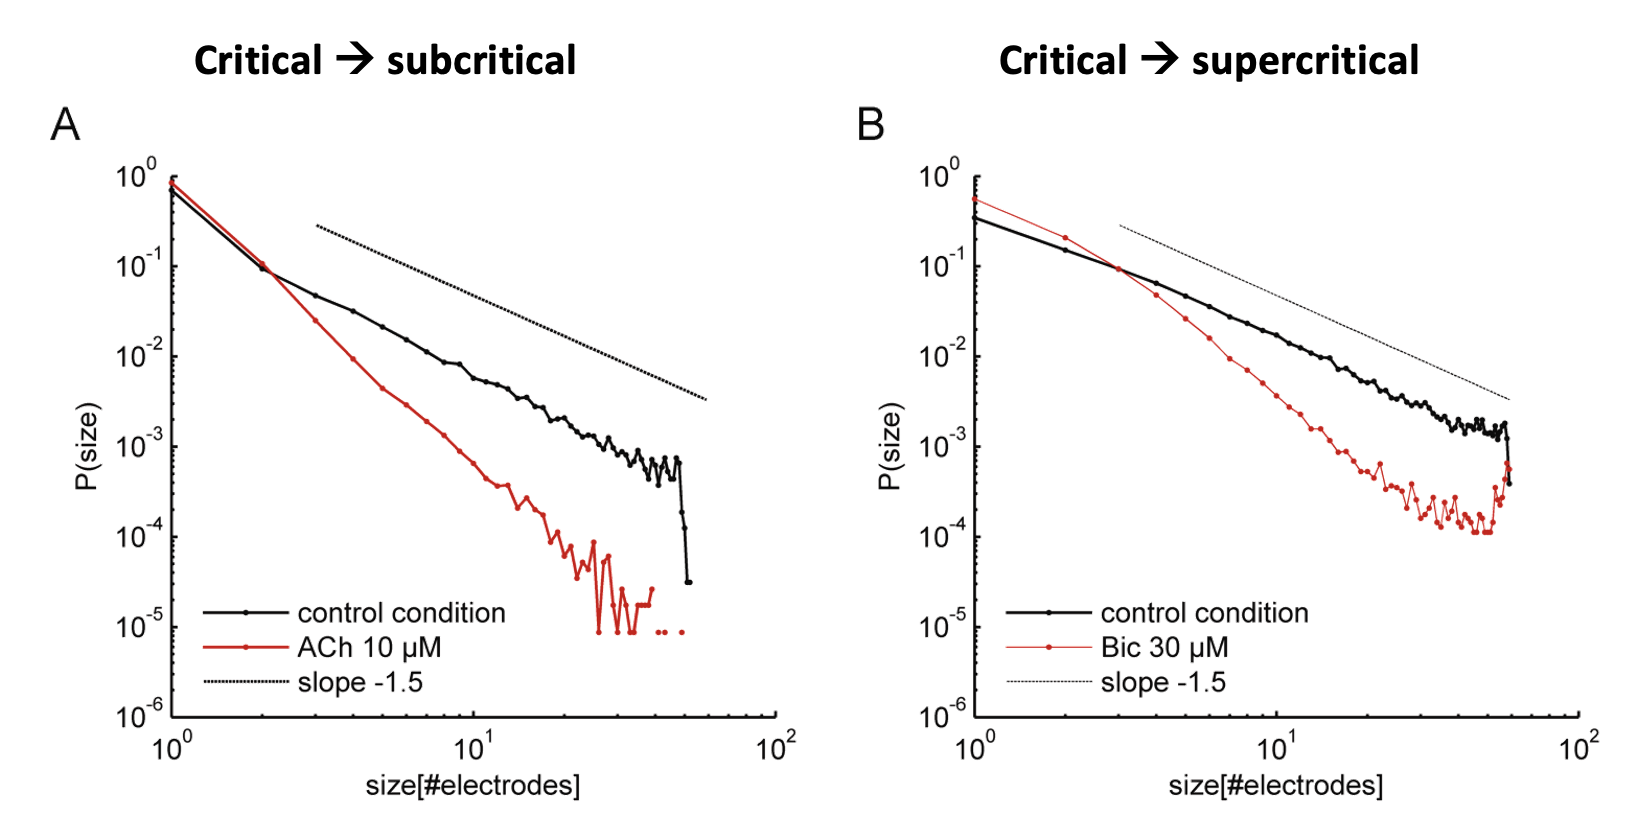
\includegraphics[scale=0.45]{8_16}
    \centering
\end{figure}
